\section{Simulation Results on Real-World Data}\label{Real_world}\thispagestyle{SectionFirstPage} % Hide headers on the first page of the section
\lhead{Simulation Results on Real-World Data}
In this chapter we will try to predict the epidemic trend based on the Covid-19 Data.

\subsection{Simulation Results}\label{figures}
\begin{figure}[H]
	\caption{USA Data}
	\centering
	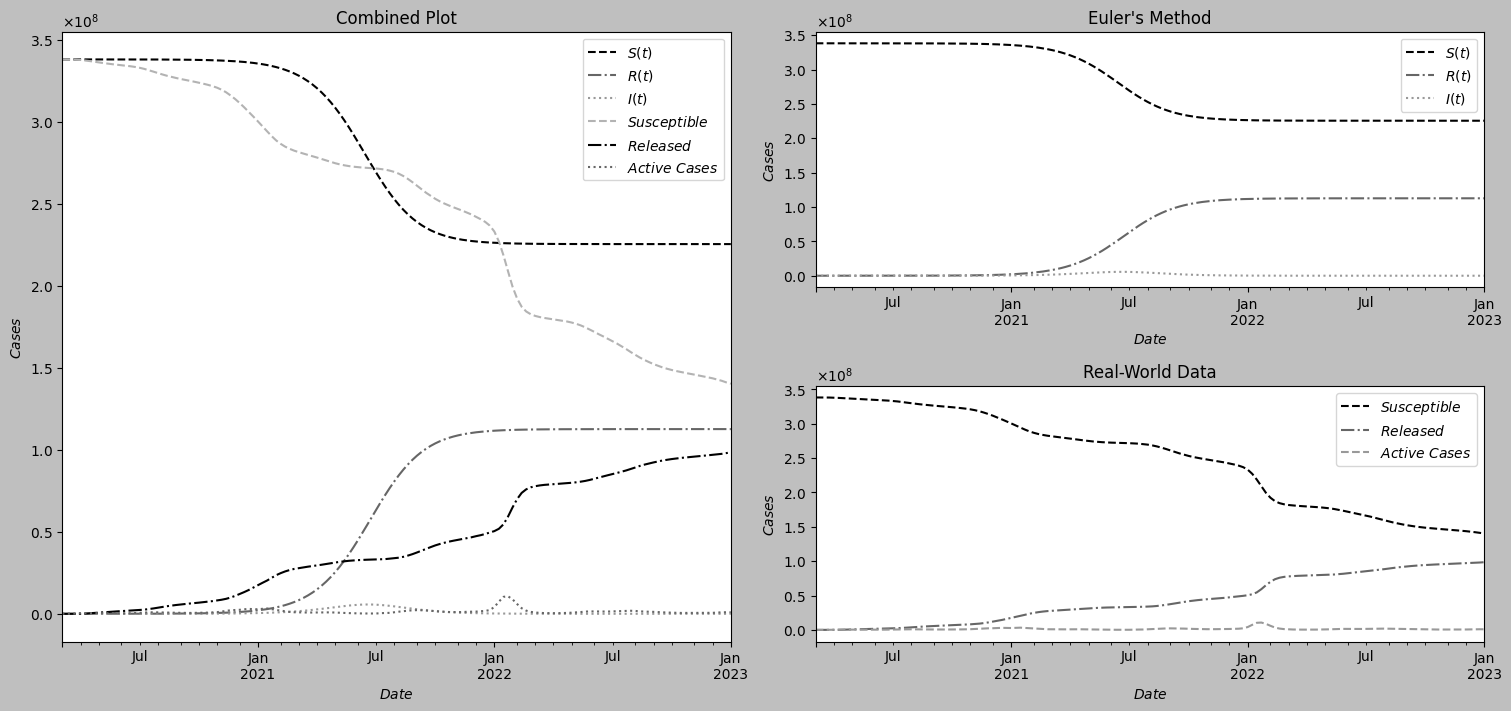
\includegraphics[width=16cm]{Figure_USAPredict.png}
\end{figure}
\begin{figure}[H]
	\caption{ARM Data}
	\centering
	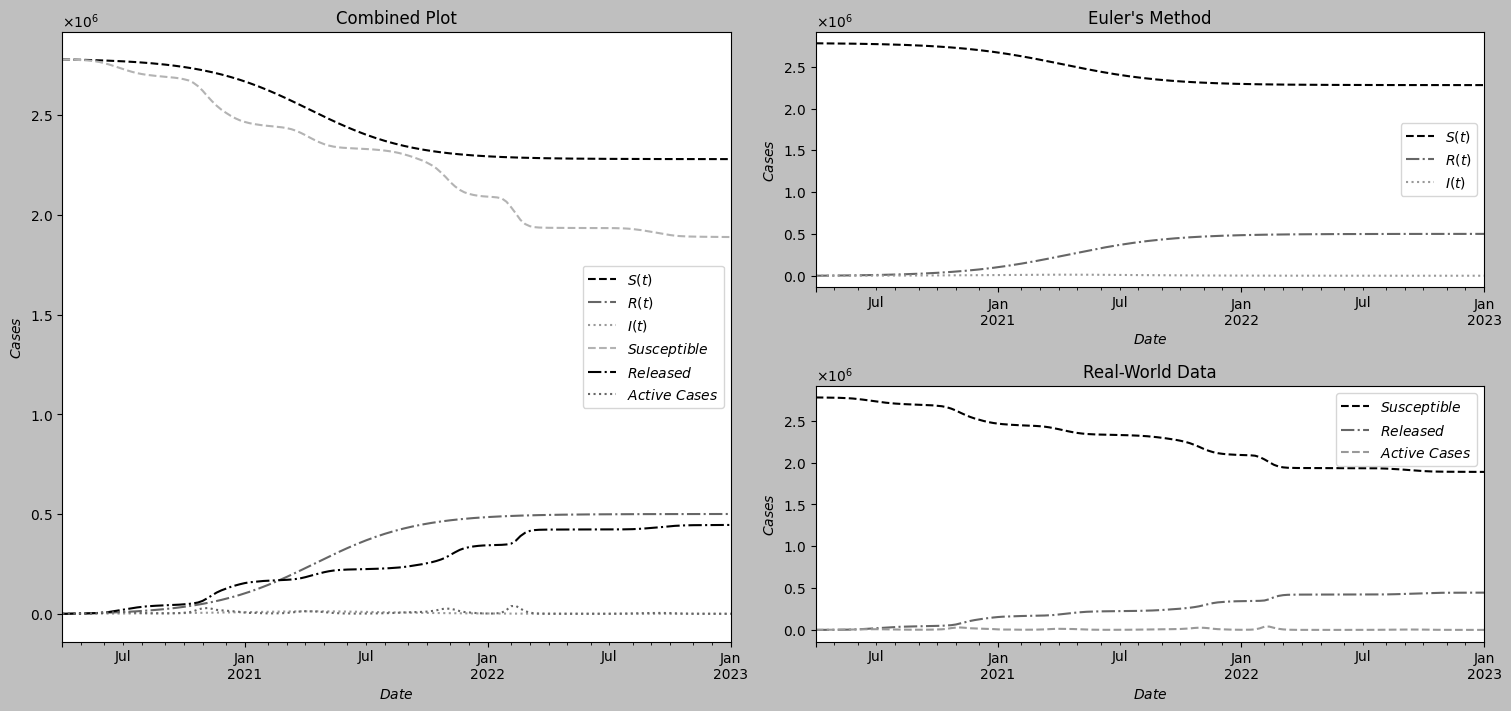
\includegraphics[width=16cm]{Figure_ArmPredict.png}
\end{figure}

\pagebreak

\subsection{Calculation \& RealWorld Use}\label{Applicaltions}
In both figures is depicted the prediction we obtained by using half the data 
of the Covid cases in their respective countries. The difficulty of predictions stems from
trying to correctly identify the optimal values for $\alpha$ and $\beta$. Firstly we need to defined what we mean 
by "optimal" values. In this case optimal was defined in a way such that the function

\begin{equation*}
	\sum_{t=0}^{n} (y(t)-y_t)^2 
\end{equation*}

is minimal. \\

Here $y(t)$ is the real world data of susceptible, infected or recovered data in time $t$. 
And $y_t$ is the point in the same time $t$ that we obtained by approximating the data with the SIR model.
Hence we want values of $\alpha$ and $\beta$ such that

\begin{equation*}
	\sum_{t=0}^{n} (S(t)-S_t)^2 + \sum_{t=0}^{n} (I(t)-I_t)^2 + \sum_{t=0}^{n} (R(t)-R_t)^2
\end{equation*}

is minimal.\\

Calculating this function for $\alpha$ and $\beta$ is a very difficult task and even the 
approximations we provided are not optimal, so we went with the brute force approach.\\
We took half the data and calculated the points for the Euler's approximation with different values for 
$\alpha$ and $\beta$. Lastly we calculated the error for each combination of $\alpha$ and $\beta$ and took 
the ones corresponding to the min of the error. What we obtained were not the most optimal values but they were still 
close. 

In Figure 2 and 3 we can see that the SIR model can to some extent predict the progression of the disease, but since the 
real world data is complex and involves a lot of other factors, it is not ideal. Those factors can include the lockdown, social distancing,
vaccines and a lot more. Hence fully predicting the progression of the diseases will not be possible, but we can still infer some useful information,
such as when approximately the diseases will plateau and what development can we expect from it in general. 